\section{Visions for Overall Change}
\label{sec:vision}
Interviewing and questioning doctors and course creators in the in-depth phase helped us focus our project. The plan for that phase was to investigate the doctors and course creators work practices, but in doing so, we discovered that the work practices at DMA regarding course promotion was the crucial point that tied the doctors and courses together.

This lead us to slightly change our focus from fitting courses into the doctors’ busy schedule, to bringing existing courses to their attention within the strict time constraints they work with.
The reason for this change was that we kept discovering new sources of medical courses that could be relevant to the doctors. There is no shortage of courses out there, so instead we focused on DMA’s unique role as an organisation. When a course is endorsed by DMA, the doctors are more likely to look at it. The challenge then is to catch the their interest and allow them to investigate these courses.

In this section, we will describe what our investigations from previous phases has led to. In particular we will talk in detail about our vision of overall change and reflect them in our prototypes.

\subsection{Technology}

Our proposed solution does not consist of creating new technologies or propose new digital platforms, but rather to use the existing systems that are available in the organisation that we have identified to play a key role in our innovation. There is, however, a coherent change in how DMA should use and approach these systems and this is where our vision comes in.

As we mentioned in the In-Depth analysis phase, the key system we found is the DMA’s newsletter and our innovations will therefore start there. The email newsletter is an existing system that DMA uses to send their members practical information. The reason for its role in our vision is that it’s accessible (i.e it doesn’t require a complicated login) and it’s perceived as one of the main channels for updates and news. Our methods are, however, by no means restricted to the newsletter, in fact we see a great potential to apply them to any distributional channels that DMA uses, such as DMA’s \fnurl{Facebook}{https://www.facebook.com/laegeforeningen} and \fnurl{LinkedIn}{https://www.linkedin.com/company/52375} pages. In this report, we will show how our proposed Hook and Reel method applies to the newsletter by referring to our prototypes which express our vision in a relative context.

\subsection{The Hook and Reel Method}
\label{hookandreel}
The name of this method is taken from the activity of fishing. The fisherman throws his hook out in the water, waits for a fish to bite and then reels it in. We thought these terms would apply very well within our project where we propose to create these so-called hooks that would get the doctors to take the bait and use the available material, i.e the act of reeling in. As with the fishing, the bait on the hook is crucial and needs to be appetising to the prey of choice, which in our case is doctors.

\subsubsection{Course Hooks}
Our vision of change proposes a distribution of hooks for courses via the newsletter (to start with). The courses behind these hooks would be a recommendation from the DMA for different specialities or for all doctors in general. A hook can be a very short video, test or other related media that doctors can use which allows them to get the sneak peek of what the course is eventually about, what the learning outcomes are and what the doctor will gain professionally from it.

The hooks are setup in such a way by including exactly how long it takes to watch, read or any other activity of participation in this introduction of the course, it allows the doctors to decide if they have any spare time to attend the course, or if the course is worth taking time out of their schedules for. In addition to that, doctors can see where and how the course takes place (e-learning course, seminar etc.) and the expected hours to finish. A mockup of how these hooks might be featured can be seen in appendix \ref{appendix:mockups}. We suggest that these hooks will be created by doctors that already have taken the course, the responsible of the course itself or even DMA itself.

\subsubsection{Course Page}
In addition to using the newsletter by promoting courses, we have also made prototypes using the Hook and Reel method, which shows our proposals of how the existing course page \ref{appendix:mockups} on DMA’s website should be updated to reflect the terms in the method. As seen in the prototype, this course page will work as a landing page where the doctor is taken to after he clicks on one of the hooks from the distribution channels. The page includes all the previous information from the hook, i.e the length of the introduction, the type of hook along with the media of the hook itself (video, test, other material) as well as additional information such as detailed description of the course, feedback from other participants and other related courses that are available.



\subsubsection{Course Feed}
Lastly, we suggest the addition of a course feed to the DMA website, where courses selected by DMA are featured. There are technical challenges with this suggestion, which will be covered in the IT systems and IT platform section, and this limits the specificity of this suggestion, but the idea is to have a list, or a feed as seen on Facebook, RSS-feeds, reddit etc., where new courses are listed. This feed can then be featured on the DMA website, either as a separate page, an addition to the front page, or as personalised feed on a “doctors page”. The feed will consist of the course hooks, and clicking on them will take you to the course page, both mentioned earlier.

The feed will be personalised based on the doctors speciality and it will include links to a “landing” page for a course.

It is important to mention that the DMA website in its current form already has course pages and an overview list. Our suggestions focus on the incorporation of the course hooks and the importance of the existence of these tools. Furthermore, the design of the current course overview requires quite a bit of time to navigate and explore. Our emphasis is again on making sure to keep the time invested for the doctors as short as possible, something we do not think the current website accomplishes.

\subsection{IT systems and IT platform}
\subsubsection{New IT system}
It should be mentioned here that DMA is currently having an entirely new website developed which will, to our understanding, completely replace the existing website frontend and backend, along with some, if not all, internal systems also. We have requested some design documents or beta access to the new system but unfortunately haven’t received any. Given this fact, we are unable to specify exactly how our prototypes will fit with the new system which is something we have had to work around.

\subsubsection{Hook creation}
As mentioned earlier, we have a few ideas on how the hooks can be created. One way would be that DMA cooperates with someone who already took the course and is familiar with the learning outcome and the professional gain of it. This would be a fair solution but probably the hardest as well. It is fair in the sense that the hook would be very familiar to the Danish doctors seeing or reading about past experience of a fellow colleague. It is, however, hard because this means that extra work is needed on top of the already busy doctor. A more realistic approach would be to cooperate with the course responsible to create the hooks. This would tie well in the current methods of work, as the course responsible would simply need to do an abstract overview of the course in a media form they consider to be the best fit. This could, for example, be an introduction test that challenges the doctor’s knowledge on some topic or an introduction video which encapsulates the scope of the course and the learning outcomes.

\subsubsection{Platform}
The platform of the hooks are not set in stone, meaning that DMA could use different platforms as they see fit. However, they do need to include some recommended features. For example, the ideal choice for a video hook would be YouTube. The YouTube video platform is very accessible, supports embedding of videos to websites and offers social media sharing. For a test hook (multi answer question hook), either using itslearning or creating some custom HTML + Javascript components that could be embedded on DMA’s website would be ideal.

\subsection{Work Organisation}
Our vision primarily aims at the work practices at DMA and specifically their role as a course promoter. The email newsletter is a key part of this process and we suggest to keep it like that with some improvements. The work related to putting courses on the website with the suggested course page is also not expected to change much in the work practices at DMA.

Creating the course hook is the biggest change to work practices. Some courses will already have a suitable course hook to use, but it remains to be seen which kind of hook works the best: videos, tests, short and concise textual introductions or other media. In any case it should be the responsibility of DMA or the course responsible to manage the production this hook.

\subsection{Qualification Needs}
For the newsletter and creating course pages, no new employee qualifications are needed except the ones dictated by the new IT-platform. For the course hook however, its creator needs to know the course and the tool to create the hook. That is why we suggest that the course responsible should have the responsibility of creating the hooks. We are suggesting using existing and well known tools and platforms for this, like YouTube for videos and itslearning for tests.


\section{Advantages and Disadvantages}
\label{sec:advantages}
\subsection{The IT Systems}
There will be no extra cost in the IT systems because we will be using the already existing IT platform that is also being upgraded, which is the Lægeforeningen website. The advantages would be that course previews on the website will be more appealing to its visitors.

\subsection{Groups of Staff and Interdepartmental Relations}
The extra cost in the work organisation would be that either someone has to be hired to create the suggested “hooks” or someone that is already involved in the promotion of the courses must also create the “hooks”. That person could be an employee of DMA, the course creators or someone that is promoting the various courses..

In terms of qualification needs, if an external company or employee is hired, it means that they will probably need to be trained to operate, or modify the existing IT systems. In case an existing employee of DMA, or a course creator is assigned to create the hooks there will not be any extra qualification needs.

\subsection{The Company’s Business and IT Strategies}
As we have stated in the previous section, there will not necessarily be any extra cost in the company business (either new employee, or existing one). The advantages will be that if the course “hooks” work the members of DMA will become more interested in the offered courses and hence continue using their membership in DMA.

In terms of the existing IT strategy, the disadvantage is that the old one will have to be discarded and so it may take some time for the current employees to adapt to the changes proposed by our innovation idea (e.g. train staff to create course “hooks”).


\subsection{SWOT analysis}
The reason that we chose to do a SWOT analysis in the last phase is because of the very limited time we’ve had available. We’ve had many innovative ideas over the course of the design process, some simple and some more complex. To help us with the decision on which idea to choose, we used this technique and chose the innovation, based on the analysis, that had the most strengths and opportunities while having fairly few threats and weaknesses. Figure \ref{fig:anal_swot} shows the identified SWOT attributes of our proposed innovation.

\begin{figure*}[h!]
 \begin{center}
  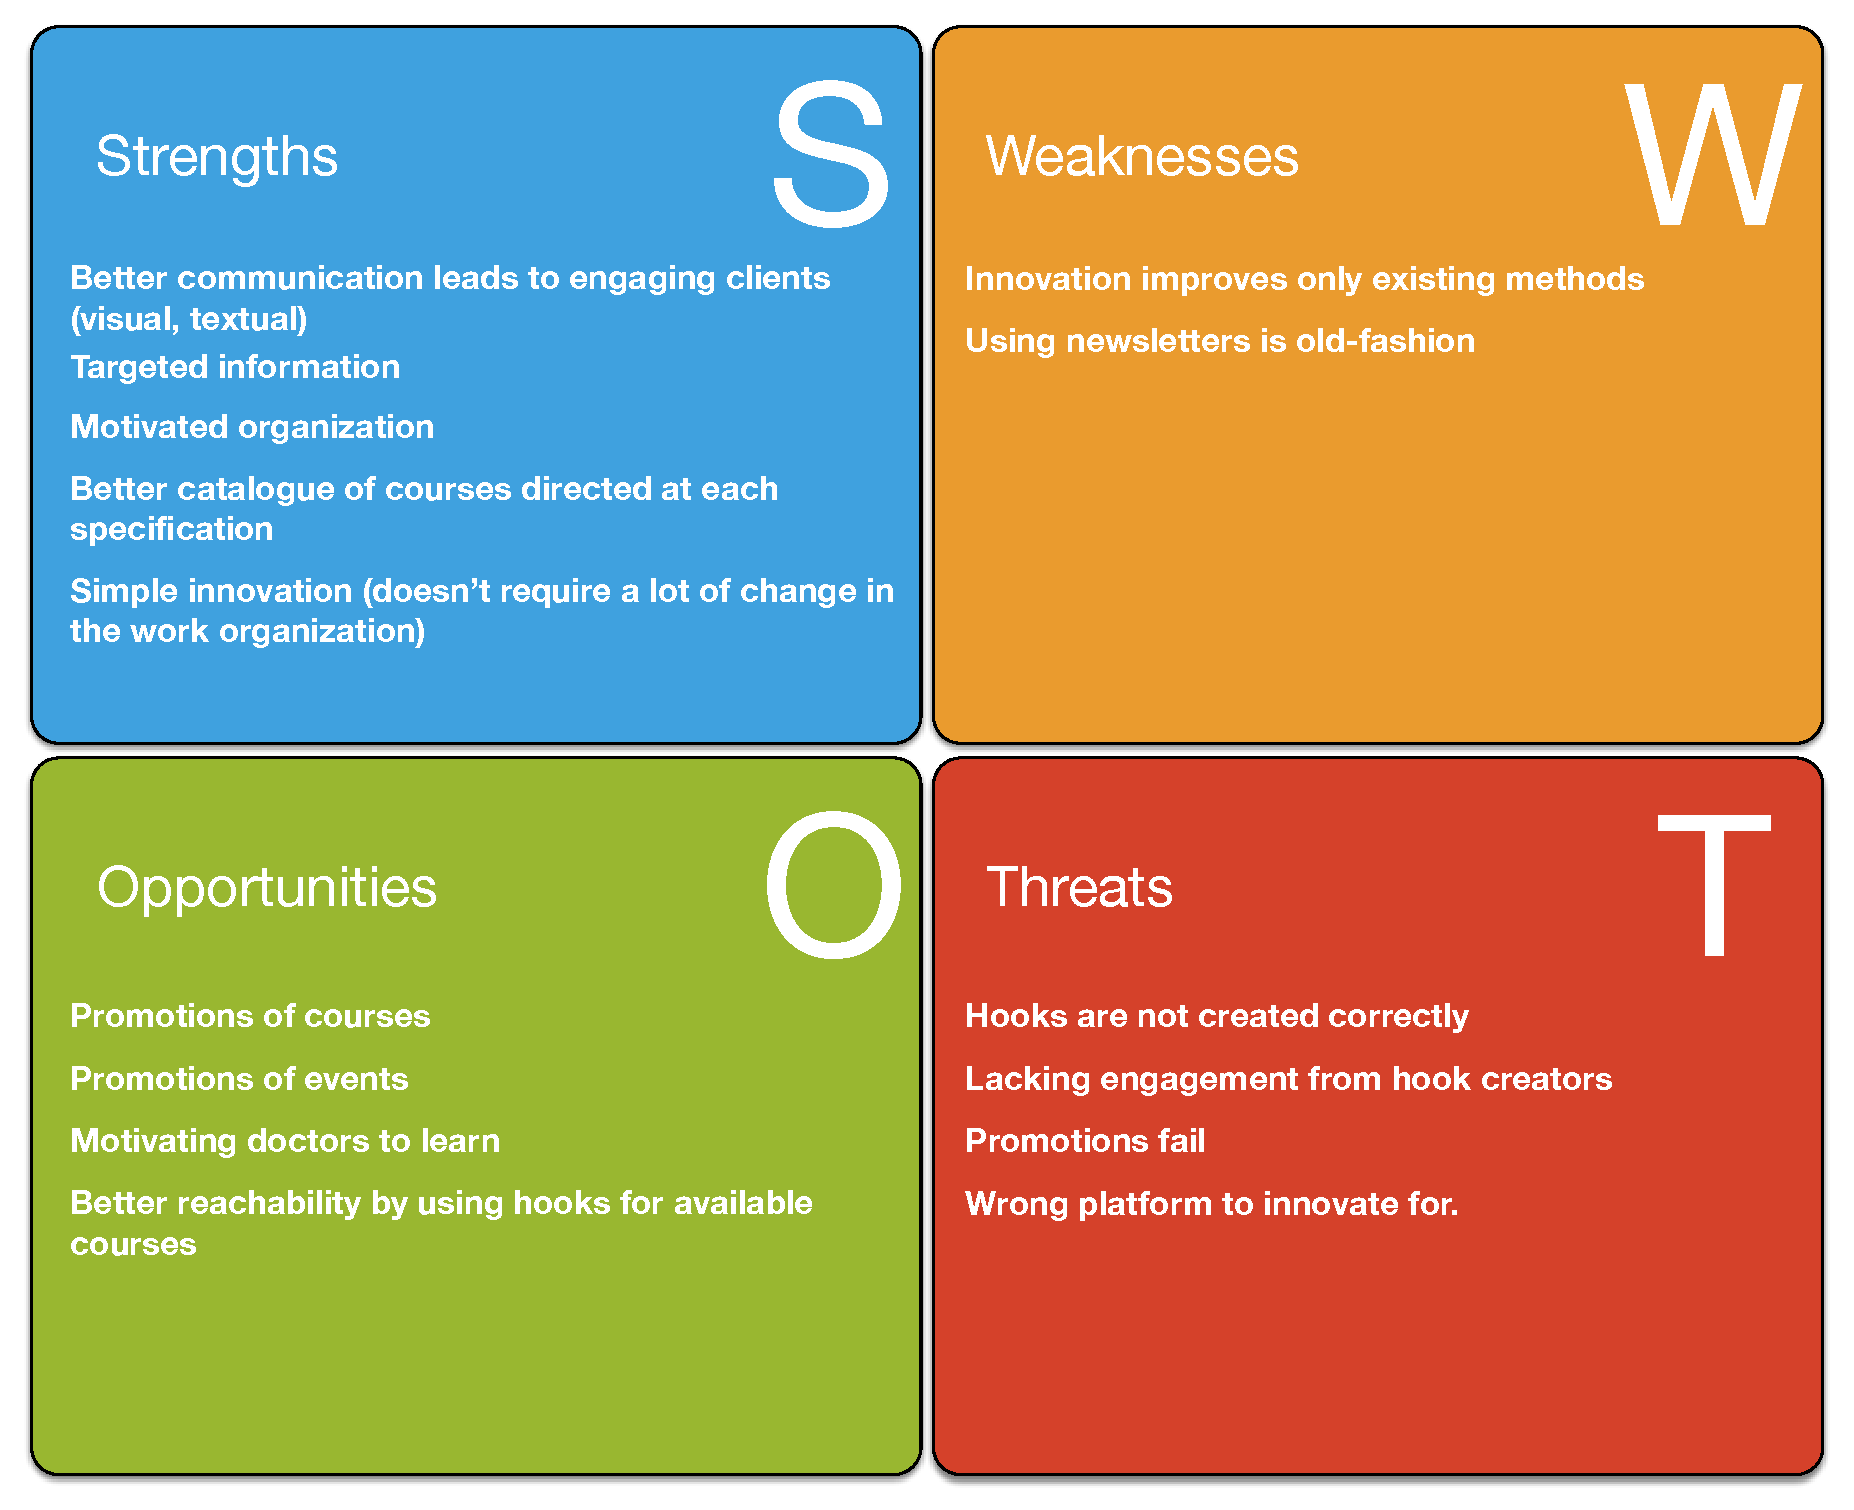
\includegraphics[width=1\textwidth]{figures/swot.pdf}
  \caption{Our baseline-plan for the project.\label{fig:anal_swot}}
 \end{center}
\end{figure*}

\subsection{Finances}
\label{sec:finances}
While this solution does not directly create a new source of income for DMA it does not really come at a great development cost either. The main expense for our innovation would be a content moderator, which DMA already employs. Meanwhile the improvements has the potential to generate value for DMA in the following ways:

\begin{itemize}
\item DMA members become increasingly satisfied with the product DMA provides and thus experiencing more value for their membership money.
\item By creating a platform with focus on a cross-channel strategy, promoting possibly both e-learning courses from partners, who are already creating the e-learning courses, such as BMJ among others, alongside traditional seminars and courses held in partnership of or by DMA, DMA has a chance to strengthen their position in the market for danish CPD courses making their members depend on them even more as a source of course providers.

This means that when DMA wants to promote their own courses they will be able to access some possibly very strong channels to advertise. This way course creators might come to depend on DMA and their platform to promote their courses, and thus ensuring their strong central position prevailing in the future. Meanwhile the increase of supply in courses available through
\end{itemize}

Given that we have moved from designing a custom e-learning solution for DMA to this promotion platform is also clearly reflected in how our Business Model Canvas for the project has changed, from being a potential source of income to instead simply generating value for DMA as seen between Figure \ref{fig:bmc1} and Figure \ref{fig:bmc2}.


\begin{figure*}[h!]
 \begin{center}
  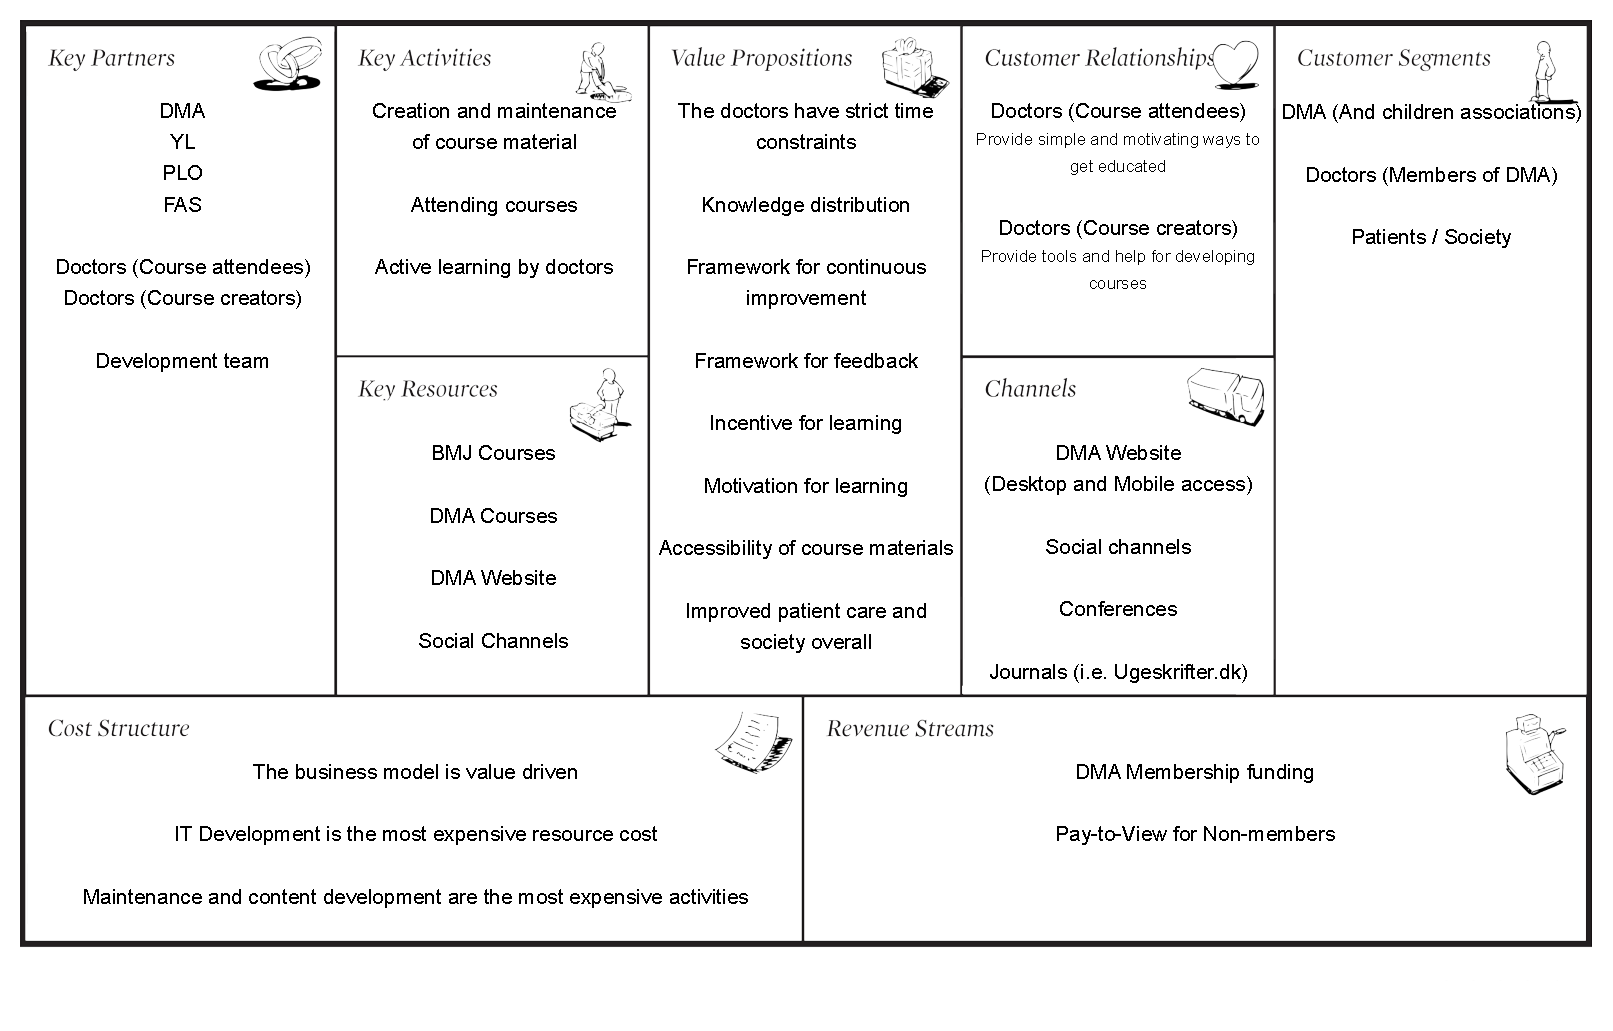
\includegraphics[width=1\textwidth]{figures/Business-Model-Canvas-v1.pdf}
  \caption{The initial BMC analysis for our project.\label{fig:bmc1}}
 \end{center}
\end{figure*}

\begin{figure*}[h!]
 \begin{center}
  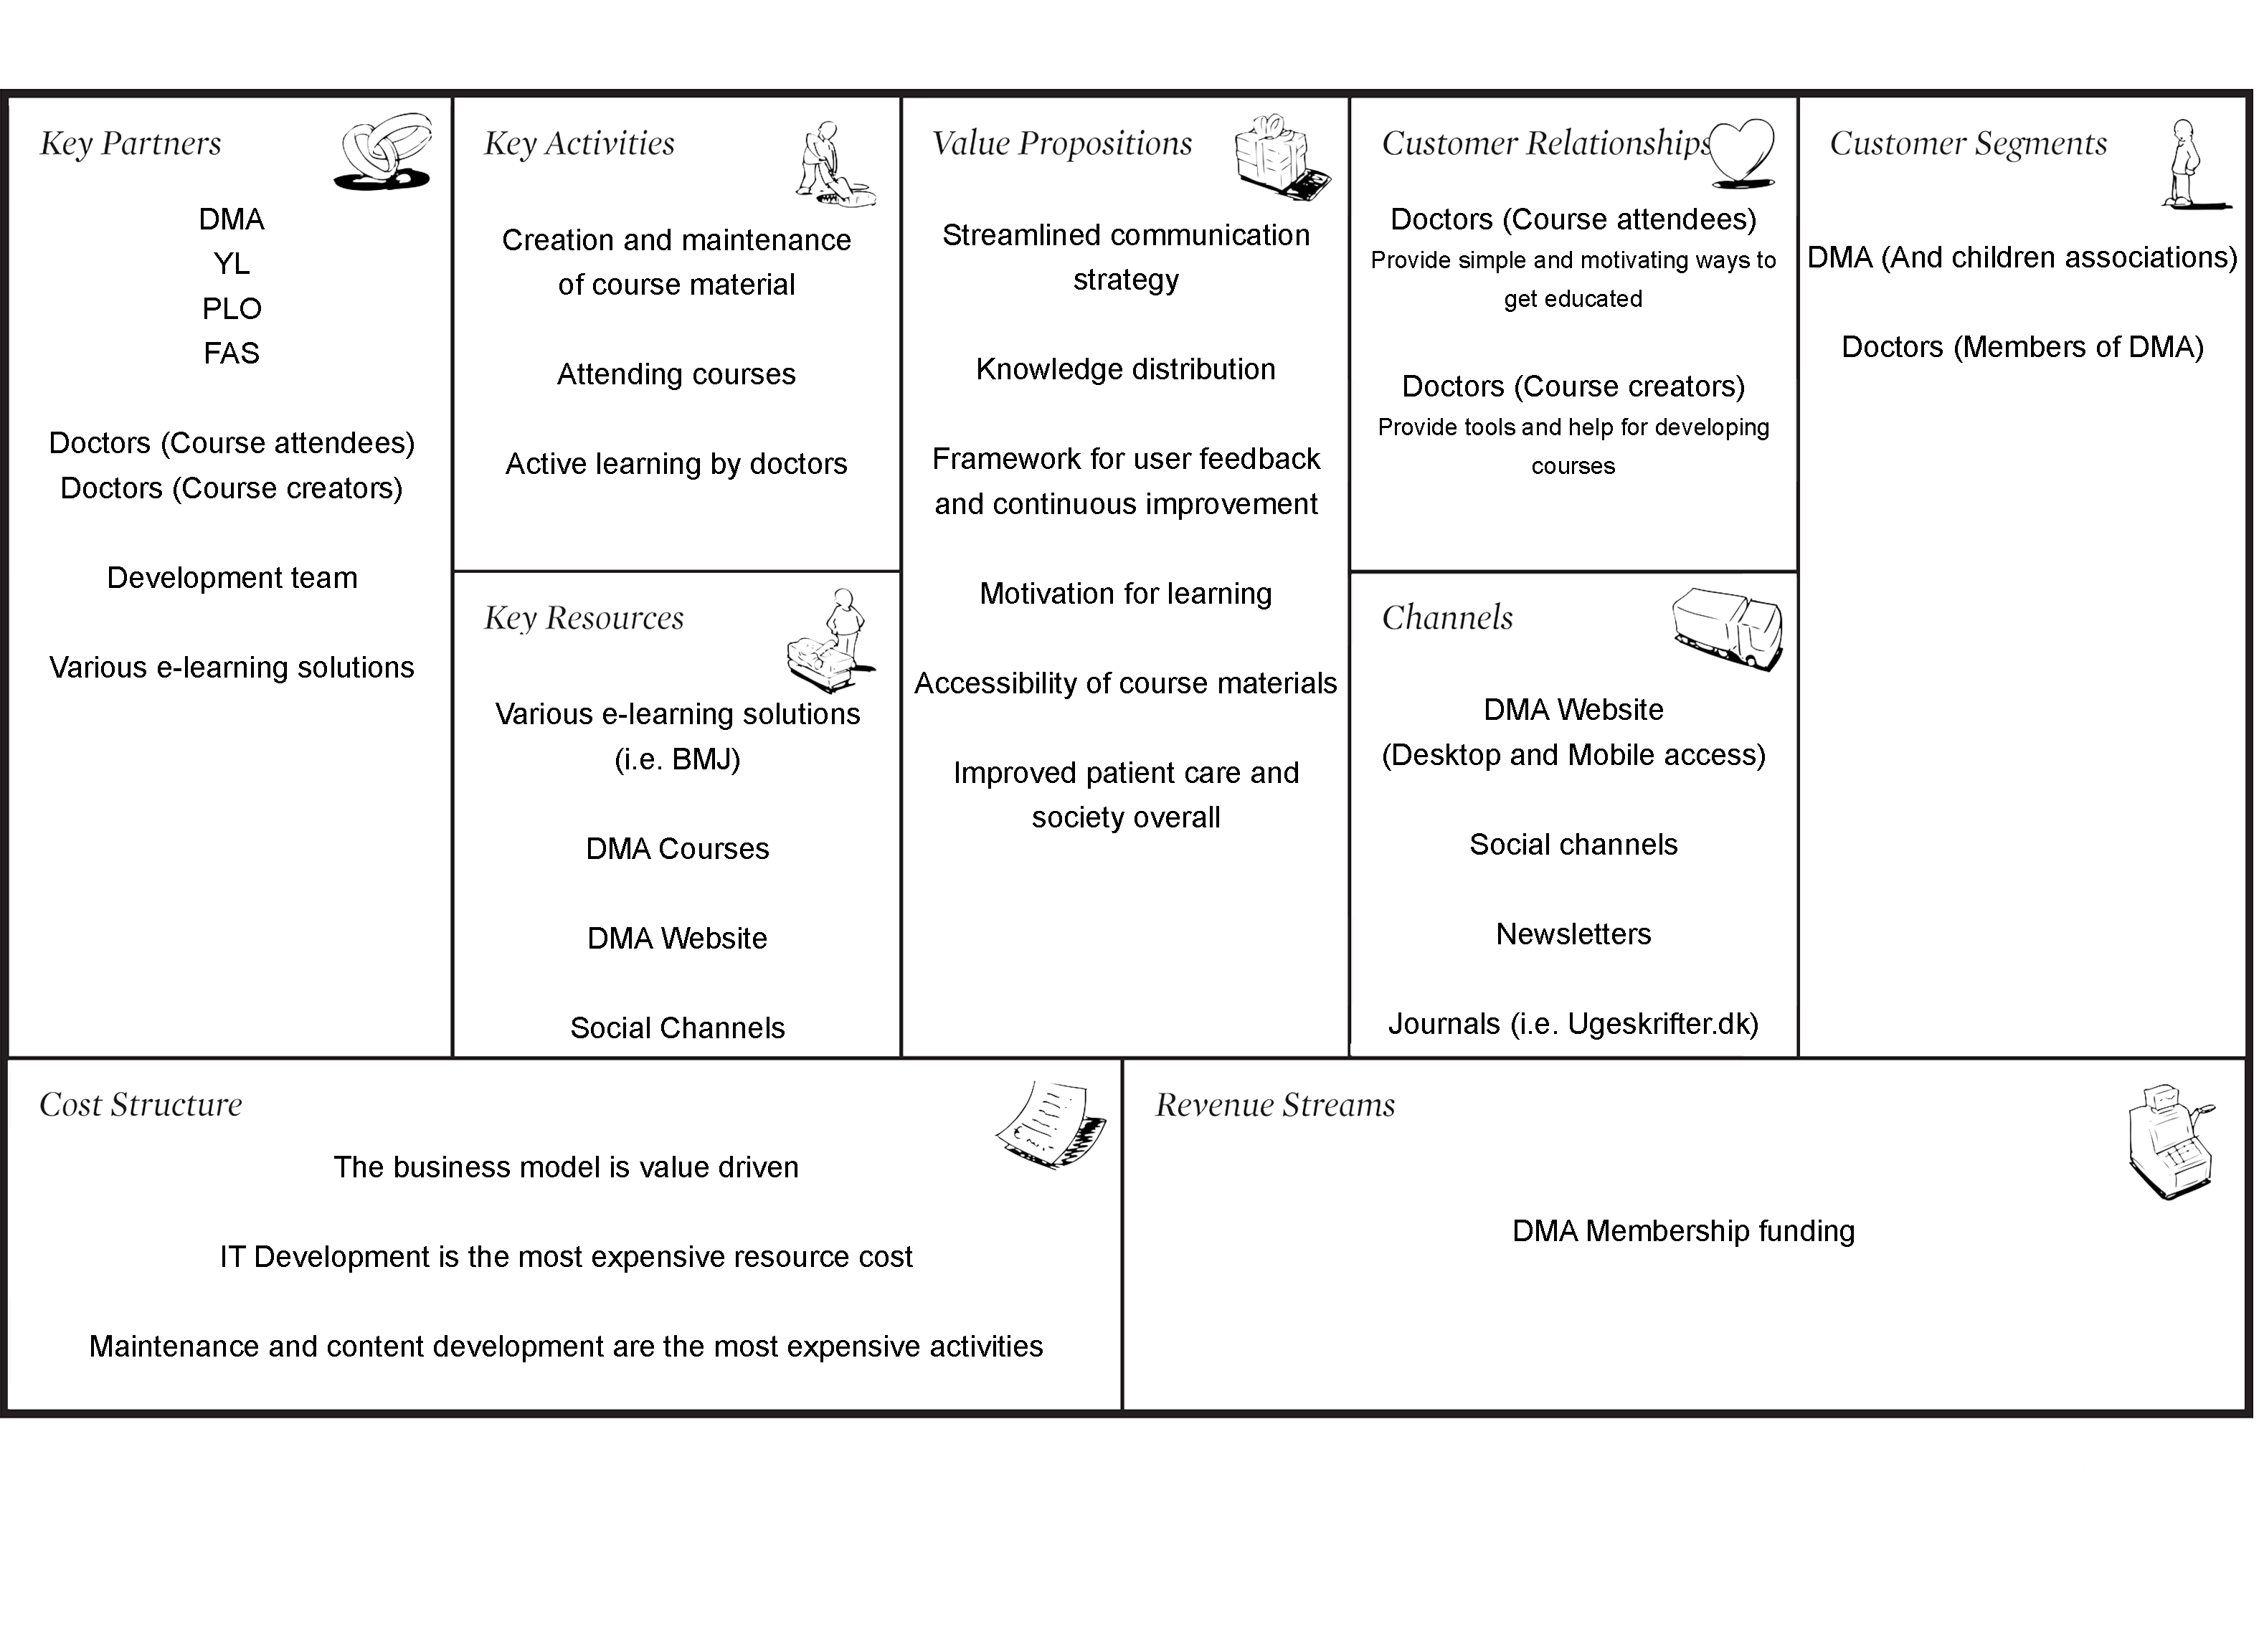
\includegraphics[width=1\textwidth]{figures/Business-Model-Canvas-v2.pdf}
  \caption{The final BMC analysis for our project.\label{fig:bmc2}}
 \end{center}
\end{figure*}
